%----------------------------------------------------------------------------
\chapter{TPSC specifikációk vizualizációja}
%----------------------------------------------------------------------------

A specifikációk vizualizációjához a \textit{Modell alapú rendszertervezés} tárgy során készített \textit{PSC} vizualizációs \textit{Sirius} alkalmazást használtam fel.
Az alkalmazással egy szerkesztő segítségével tudunk \textit{PSC} diagramokat rajzolni.
Egy palettáról lehet kiválasztani az egyes elemeket és az egérrel elhelyezni őket a diagramon.
Ezután pedig megadhatók a paramétereik, például egy üzenetnél, hogy melyik objektum a küldője és fogadója, vagy hogy milyen megkötések vannak rajta, egy objektumnál, hogy mi a neve és típusa.
A \ref{sirius_psc} ábrán megtekinthető a paletta és néhány példa diagram.

\begin{figure}[!ht]
    \centering
    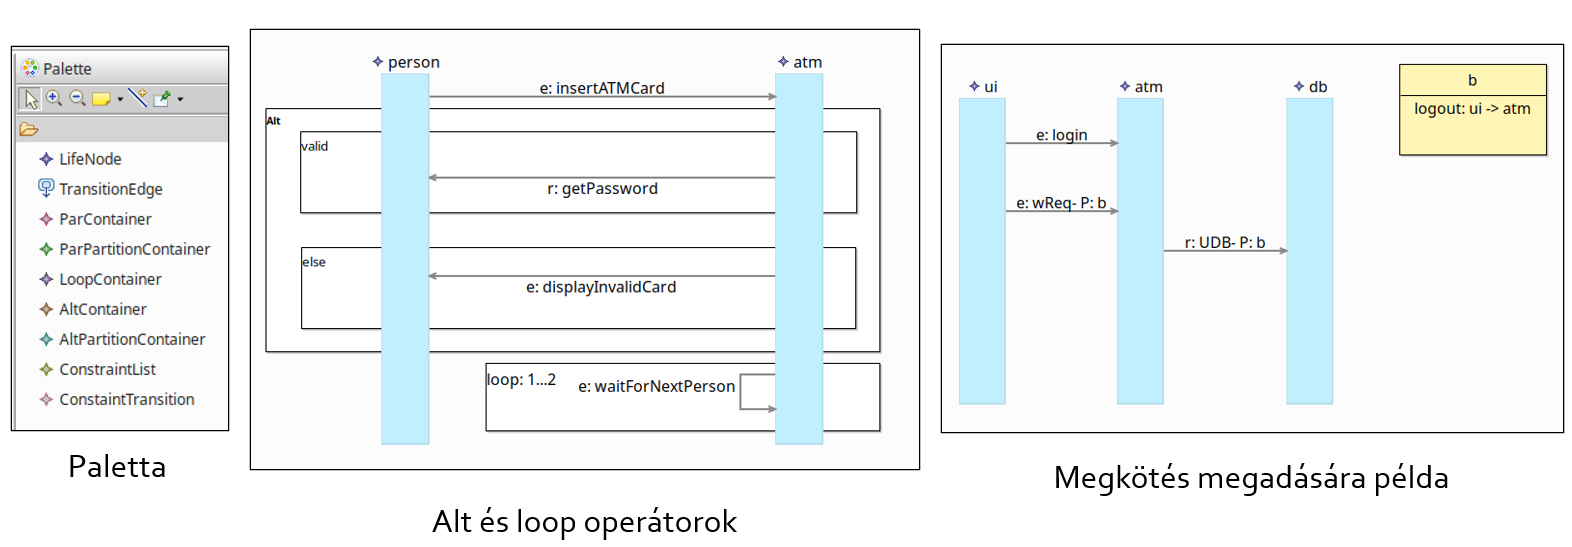
\includegraphics[width=150mm, keepaspectratio]{figures/sirius_psc.png}
    \caption{\textit{PSC} vizualizációs alkalmazás bemutatása.}
    \label{sirius_psc}
\end{figure}

Először kiegészítettem az alkalmazást \textit{TPSC} elemek vizualizációjával.
Ehhez az alkalmazáshoz tartozó \textit{EMF} modellben fel kellett vegyem, hogy egy üzeneten elhelyezhető legyen időzítési feltétel is.
Ezt ugyanígy meg kellett tegyem a megkötéseknél is és ezen kívül az óraváltozók nullázását is hozzáadtam a modellhez.
Ezután a vizualizációhoz hozzáadtam, hogy az időzítési feltétel és az óraváltozó nullázása megjelenjen az átmenetek címkéin.
Készítettem egy \textit{Xtend} alapú \textit{XML} generátort, ami képes a szöveges \textit{TPSC} leírás alapján legenerálni a hozzá tartozó \textit{XML} leírást.
Ezt a leírást képes a \textit{Sirius} alkalmazás feldolgozni és előállítani a hozzá tartozó diagramot.
Egy ilyen generált \textit{XMl} fájl megtekinthető a \ref{sirius_xml} kódrészleten.

\begin{lstlisting}[language=java, frame=single, float=ht!, caption={Szcenárió szöveges leírása.},captionpos=b, label=sirius_tpsc_text]
specification Email{

    object Computer computer;
    object Server server;

    integer timeout = 10;
    string receiver = "John";
    string subject = "Next meeting";

    clock x;

    constraint constraints {
        message logout() computer -> server;
    }

    scenario sendEmail{
        message checkEmail() computer -> computer reset x;
        required message sendUnsentEmail() computer -> server;
        pastConstraint {constraints} message newEmail(receiver, subject) computer -> server;
        message downloadEmail(timeout) computer -> server clockConstraint {>(x,10)};
    }
}
\end{lstlisting}

\begin{figure}[!ht]
    \centering
    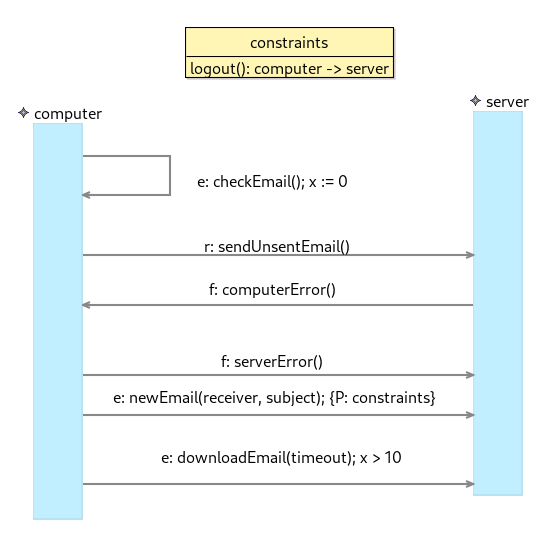
\includegraphics[width=100mm, keepaspectratio]{figures/diagramExample.png}
    \caption{\textit{Sirius} által előállított szcenárió diagram.}
    \label{sirius_diagram}
\end{figure}

\begin{lstlisting}[language=java, frame=single, float=ht!, caption={Szenárió diagram xml leírása.},captionpos=b, label=sirius_xml]
<?xml version="1.0" encoding="UTF-8"?>
<minotor:SequenceDiagram xmi:version="2.0" xmlns:xmi="http://www.omg.org/XMI" xmlns:minotor="hu.bme.mit.mdsd.xboyz.erdiagram" Name="Email">

<lifelines Name="computer" Type="Computer"/>
<lifelines Name="server" Type="Server"/>

<constraints Name="constraints">
<transitions Name="logout()" source="//@lifelines.0" target="//@lifelines.1"/>
</constraints>

<transitions Name="checkEmail()" Type="REGULAR" Label="e: checkEmail()" source="//@lifelines.0" target="//@lifelines.0"  after="//@transitions.1" reset="x"/>
<transitions Name="sendUnsentEmail()" Type="REQUIRED" Label="r: sendUnsentEmail()" source="//@lifelines.0" target="//@lifelines.1" before="//@transitions.0" after="//@transitions.2"/>
<transitions Name="computerError()" Type="FAIL" Label="f: computerError()" source="//@lifelines.1" target="//@lifelines.0" before="//@transitions.1" after="//@transitions.3"/>
<transitions Name="serverError()" Type="FAIL" Label="f: serverError()" source="//@lifelines.0" target="//@lifelines.1" before="//@transitions.2" after="//@transitions.4"/>
<transitions Name="newEmail(receiver, subject)" Type="REGULAR" Label="e: newEmail(receiver, subject)" source="//@lifelines.0" target="//@lifelines.1" before="//@transitions.3" after="//@transitions.5" constraint="//@constraints.0" constraintType="PAST"/>
<transitions Name="downloadEmail(timeout)" Type="REGULAR" Label="e: downloadEmail(timeout)" source="//@lifelines.0" target="//@lifelines.1" before="//@transitions.4"   clockConstraint="x &gt; 10"/>
</minotor:SequenceDiagram>
\end{lstlisting}

A vizualizációs diagramon az egyes objektumok kék \textit{lifeline} formájában jelenek meg.
Minden üzenethez tartozik egy nyíl, amely címkéjére írjuk az üzenet összes tulajdonságát.
Például a megkötések '\{' '\}' jelek között jelennek meg.
Egy \textit{P} betű jelöli, hogy a megkötés múltbéli és egy \textit{F} betű ha jövőbeli.
A nyíl eleje és vége \textit{lifeline}-okat kötnek össze, amik az üzenet feladóját és fogadóját jelzik.
A megkötéseket egy sárga táblázat formájában reprezentáljuk, amelybe bele írjuk az összes megkötésben szereplő üzenetet.
Egy ilyen diagramot mutat be a \ref{sirius_diagram} ábra.
A diagram szöveges leírását pedig a \ref{sirius_tpsc_text} kódrészlet tartalmazza.
%Az alkalmazáshoz tartozó \textit{ER} diagram a \ref{er_diagram} ábrán található meg.

%\begin{figure}[!ht]
%    \centering
%    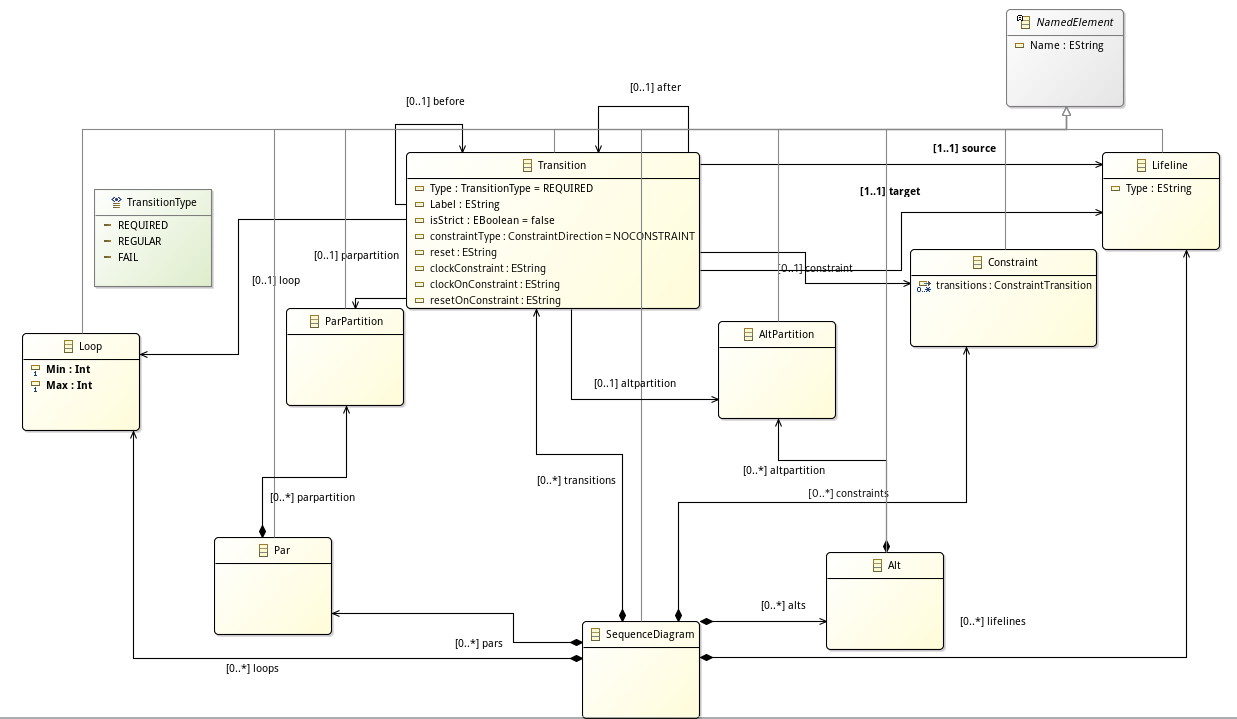
\includegraphics[width=150mm, keepaspectratio]{figures/sirius-minotor-erdiagram.png}
%    \caption{\textit{Sirius} alkalmazáshoz tartozó modell \textit{ER} diagramja.}
%    \label{er_diagram}
%\end{figure}

\begin{figure}[!ht]
    \centering
    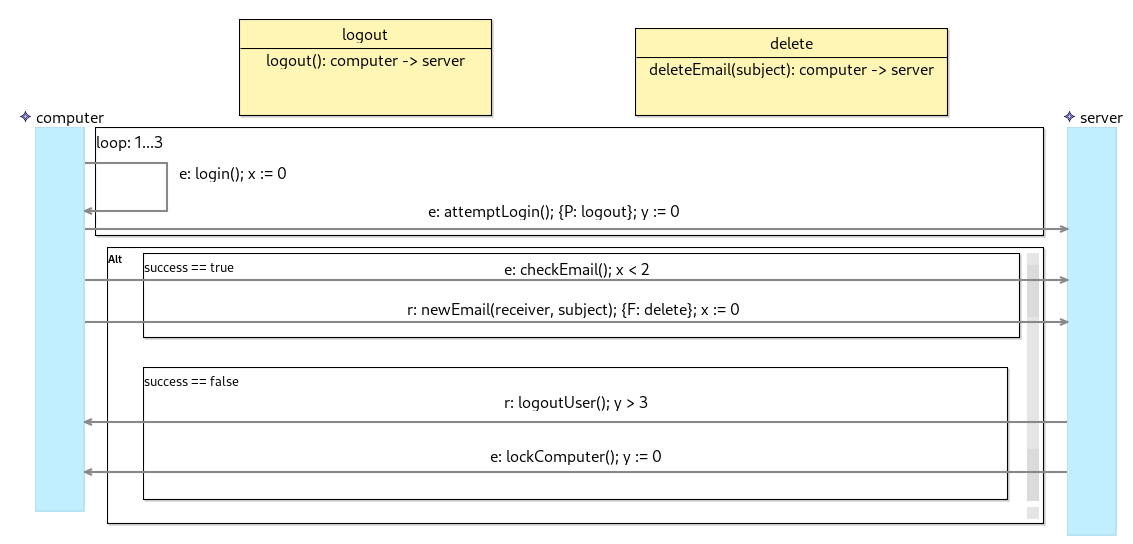
\includegraphics[width=150mm, keepaspectratio]{figures/diagramOperatorExample.png}
    \caption{Operátorokat tartalmazó szcenárió diagram.}
    \label{sirius_operators}
\end{figure}

A diagramon keretek formájában jelenek meg az operátorok.
Ilyen operátorokat a \ref{sirius_operators} diagramon lehet megtekinteni.